

\subsection{Trigger}
\label{sec:trigger}

The nominal instantaneous luminosity is around $2\times10^{32}\cm^{-2}\sec^{-1}$ during Run 1 and Run 2,  
and the rate of events with collisions is roughly 10 \mhz 
when produce at least two charged particles with enough \velo and tracking hits to allow for their reconstruction. 
In fact, 
the rate to storage is about 2-5 \khz,
which is achieved by the trigger system to reduce the rate by selecting only interesting events.
An intial reduction down to 1 MHz comes from the Level-0 (\lone) hardware trigger, 
which uses custom electronics and runs synchronously with the 40 MHz bunch crossing frequency. 
High Level Trigger (\hlt) follows the \lone,
which is a software-base trigger.
The \hlt is subdivided into two stage,
which runs asynchronously on a processor farm and reduces the rate to the desired range. 
The \lhcb trigger scheeme is shown in Figure.~\ref{fig:TRIGGER}.
More details will be given on each stage in the following sections.

\begin{figure}[!hbtp]
\centering
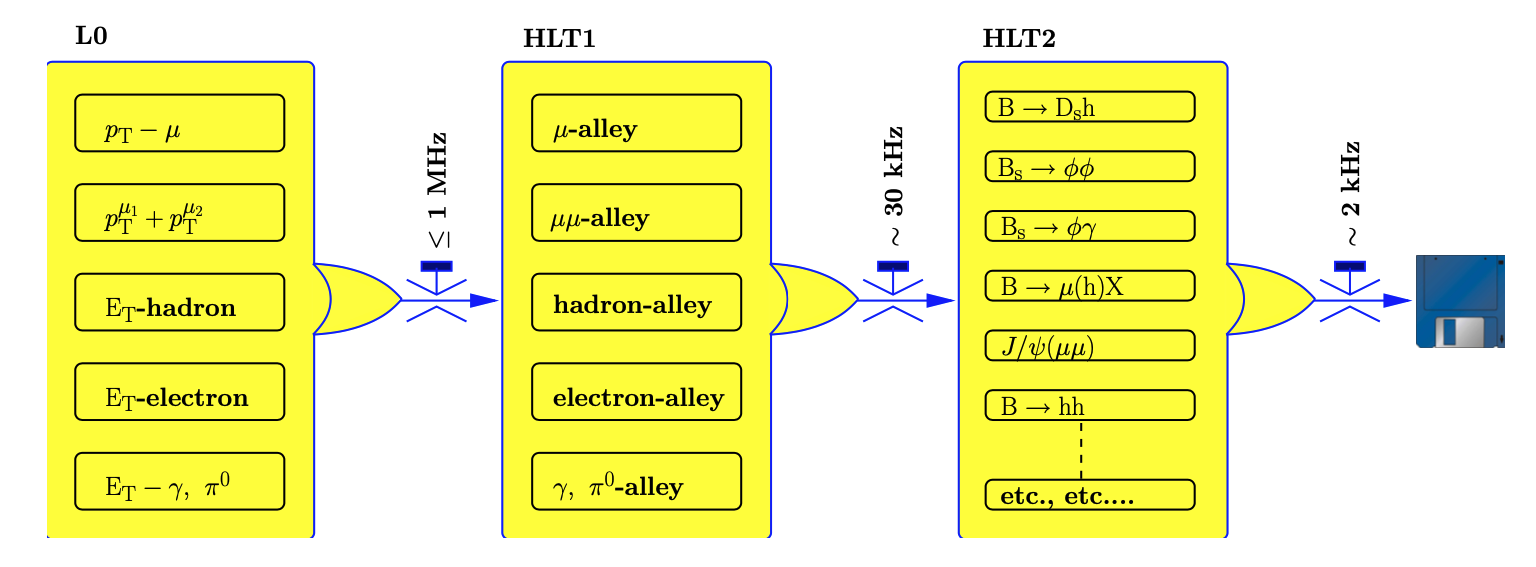
\includegraphics[width=0.99\textwidth]{Figures/02_Detector/TRIGGER}%
\caption{ Flow-diagram of the different trigger sequences\supercite{LHCb-DP-2008-001}.}
\label{fig:TRIGGER}
\end{figure}


\subsubsection{\lone trigger}

The \lone trigger contains three components:
the pile-up system,
the Level-0 calorimeter trigger and the Level-0 muon trigger.
All components are connected to the Level-0 dicision unit (DU) 
which is used to evaluate the final dicision by collecting all the information obtained from the trigger system,
as shown in Figure.~\ref{fig:L0_trigger}.

\begin{figure}[!hbtp]
\centering
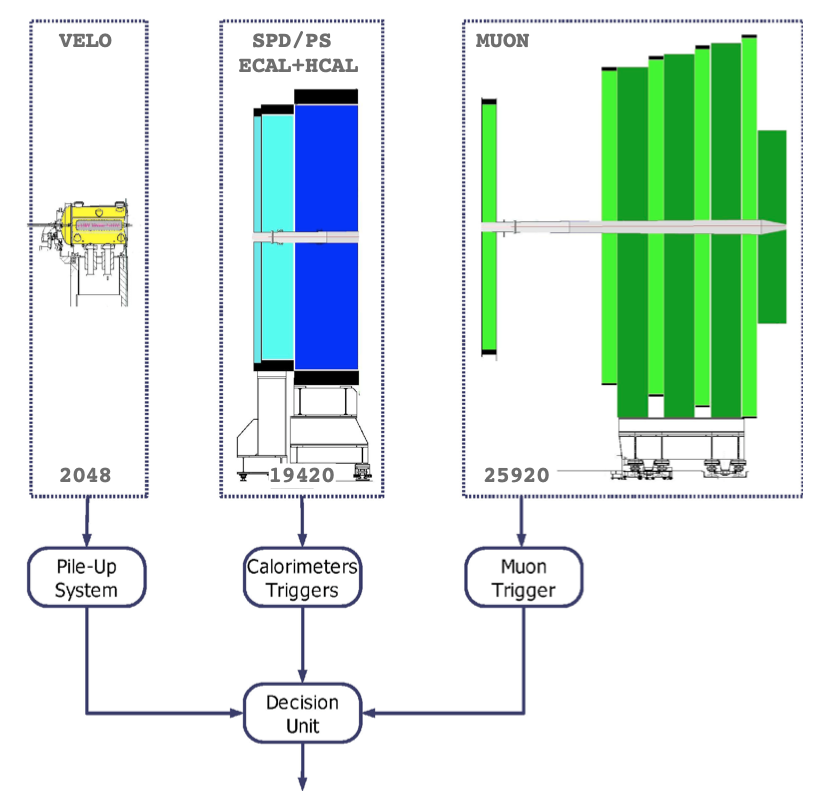
\includegraphics[width=0.49\textwidth]{Figures/02_Detector/L0_trigger}%
\caption{ Overview of the \lone trigger\supercite{LHCb-DP-2008-001}.}
\label{fig:L0_trigger}
\end{figure}

The pile-up system is used to distinguish the crossings with single and multiple visible interactions, 
which is based on the silicon sensors in the \velo to measure the radial position of tracks. 
The pile-up system has two functions: 
to provide the position of the primary vertices candidates along the beam-line 
and to measure of the total backward charged track multiplicity.


The calorimeter trigger is designed to search for high \et particles by adding the \et of $2\times2$ cells and selecting the clusters 
with the largest \et,
this step is performed on the Front-End card.
Then the information from \ecal and $\presh \& \spd$ are merged to identifiy the type of electromagnetic candidate, electron, $\gamma$ or \piz.
Besides,
the \et of all \hcal cells is summed to reject crossings without visible interactions. 
The total number of \spd cells with a hit are counted to provide a measure of the charged track multiplicity in the crossing.
%Besides, 
%measurements of the total \et in \hcal and total \spd multiplicity are also performed.

A \lone muon processor is used to search for the two muon tracks with the largest and second largest \pt,
which is performed on the logical pads.
This trigger can look for hits regarded as a straight line through the five muon stations and pointing to the interaction point.
The track position in the first two stations allows the determination of its \pt.
From this system, 
the \pt resolution of a reconstructed stand-alone muon can reach to ~$20\%$.


\subsubsection{\hltone trigger}

The \hltone trigger can reconstruct the trajectories of charged particles traversing full \lhcb tracking system,
besides,
a precision primary vertex reconstruction is perform\supercite{Aaij_2019}
Most particle-identification algorithms cannot be executed in this stage excepting muon identification,
due to a clean signature.
At the same time,
the electrons are identified by associating tracking to \ecal clusters,
photon and neutral pion are also built fromt he clusters reconstructed in the \lone trigger.

The steps of \hltone algorithms is shown in Figure.~\ref{fig:Hltone}.
Firstly, 
the \velo tracks are reconstructed,
as well as the finding of primary vertices.
Then the \velo tracks are extraploted to match the hits in the \ttracker stations to form upstream tracks.
By the way, 
this process can also reduce the number of fake \velo tracks.
Finally, 
the long tracks are reconstructed by combining the information from downstream trackers,
and the search window in the \intr and \ot is defined by the maximum possible function of charged particles with \pt larger than $500\mev$.
The next step is to fit tracks with a Kalman filter to obtain the optimal parameter estimate,
as well as the fake track rejection to removed the tracks with poor quality.

\begin{figure}[!hbtp]
\centering
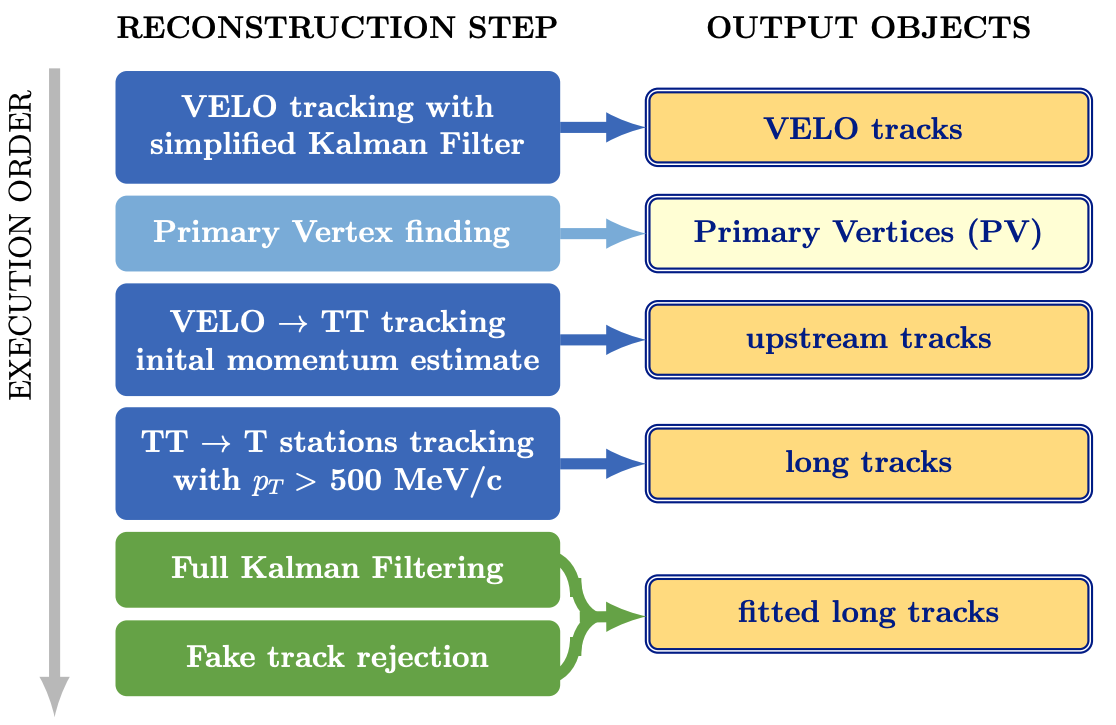
\includegraphics[width=0.69\textwidth]{Figures/02_Detector/Hltone}%
\caption{Track and vertex reconstruction in the \hltone trigger\supercite{Aaij_2019}.}
\label{fig:Hltone}
\end{figure}

The muon identification in \hltone with all fitted tracks.
For the muon tracks,
the corresponding hits are required in the fout MUON stations,
which is also used in \hlttwo and offline.


\subsubsection{\hlttwo trigger}

In the \hlttwo stage,
the full event reconstruction and identification is performed,
including the charged track reconstruction,
neutral particle reconstruction and particle identification with the information from PID detectors considered.
The corresponding steps of track and vertex reconstruction are shown in Figure.~\ref{fig:Hlttwo}.

\begin{figure}[!hbtp]
\centering
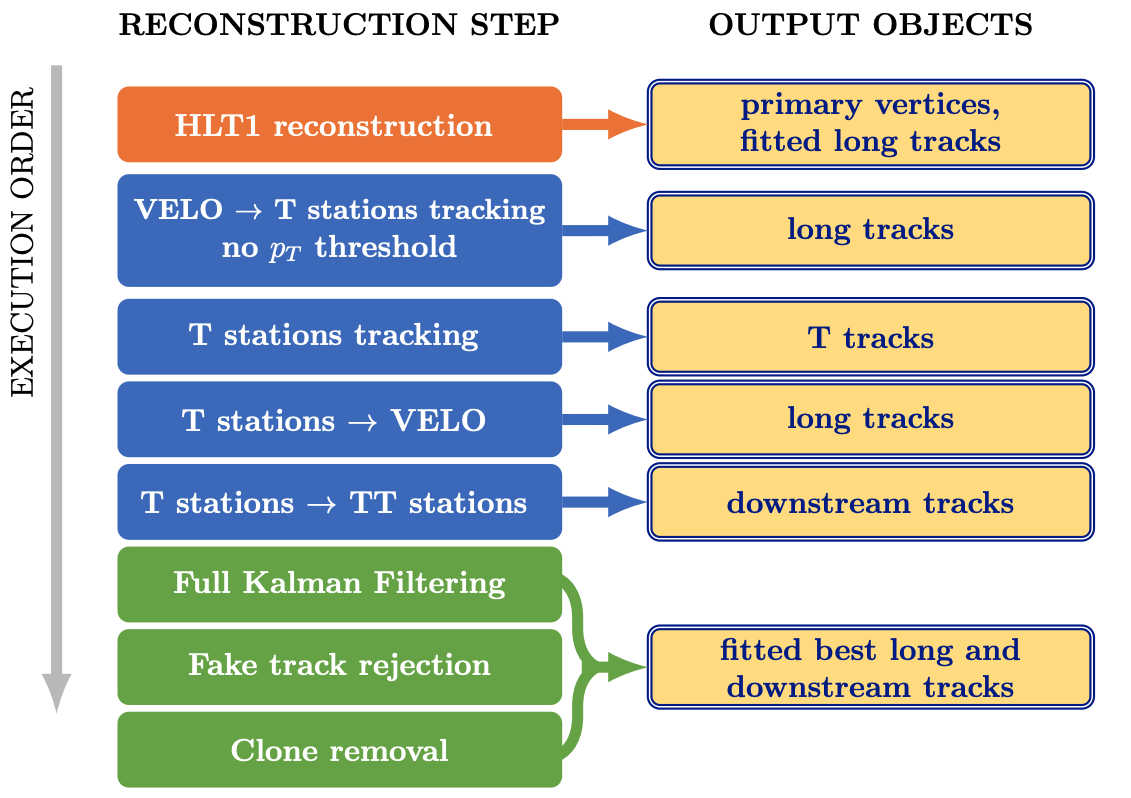
\includegraphics[width=0.69\textwidth]{Figures/02_Detector/Hlttwo}%
\caption{Track and vertex reconstruction in the \hlttwo trigger\supercite{Aaij_2019}.}
\label{fig:Hlttwo}
\end{figure}

In the charged particle reconstruction process,
the \hltone algorithm is repeated firstly,
a second step is to reconstruct the lower-momentum tracks with is overlooked in \hltone.
The track reconstruction becomes larger as low \pt tracks included and no \ttracker hits required.
Besides,
the long-live particles that decay outside the \velo are reconstructed using T-station segments,
which are extrapolated to the magnetic field and combined with hits in the \ttracker.
Next step is to reject fake tracks from the random combination of hits or a mismatch with different tracks segments.
This procedure is based on the Kalman filter and multi-variable analysis tool (TMVA).
Then the remaining tracks are filtered to remove the clone tracks that share enough hits in each subdetector.

The \rich detectors provide the important discrimination between kaons, pions and protons,
and this information can add likelihood for each mass hypothesis to the reconstructed tracks.
The calorimeter system can offer PID information by matching between reconstructed tracks and calorimeter clusters,
combining the information from MUON system,
mature PID values are provided to the tracks.


\subsubsection{Trigger system after \upgradeone}

The most distinguishing feature of trigger after \upgradeone at \lhcb is a full software scheme,
which can offer unprecedented flexbibility in designing selections, 
and in particular allows efficient triggering on low-momentum signatures wich would normally be out of the reach for hadron collider.
The dataflow after \upgradeone is illustrated in Figure.~\ref{fig:Hlt_upgrade}

\begin{figure}[!hbtp]
\centering
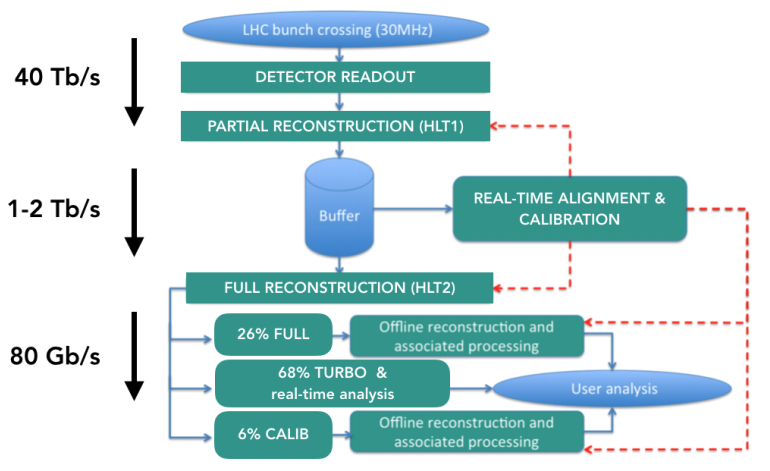
\includegraphics[width=0.69\textwidth]{Figures/02_Detector/upgrade_trigger}%
\caption{Dataflow in the upgraded \lhcb detector\supercite{LHCb-TDR-021}.}
\label{fig:Hlt_upgrade}
\end{figure}

%The all trigger system after \upgradeone consists several steps.
%Firstly,
%the data collected from subdecters are processed in event filter farm (EFF) using the RTA applications,

As the \lone trigger is removed,
all the tigger dicisions are based on the \hlt,
which is split into two stages, 
as similar as the strategy in Run 2.
This two stages is seperated by a disk buffer that save data used for alignment and calibration.
The \hltone can reject events contain only poor intesting particles for any \lhcb analysis,
and \hlttwo use the full reconstruction and identification algorithms to obtain the high-level physics objects relevant to analysis for permanent storage.
Many R\&D projects are under way currently,
and some algorithm optimization and code migration tasks have made great advances\supercite{LHCb-TDR-021,LHCb-TDR-018,LHCb-TDR-017,LHCb-TDR-016}.























